\section{User Experience for mobiles}
\subsection{Introduction to user experience }
A study of user experience\footnote{hereafter referred to as UX} is a study of how a user feels when interacting with a system. The field encompasses a whole range of different and seemingly unrelated topics. The most known part of UX is probably the concept of usability which will be discussed later in the chapter, other things makes up UX, such as: Design, Accessibility, System performance, Ergonomics, human factors and more concept. The term user experience  was originally coined by Dr. Donald Norman, who was the first to describe the importance of user-centered design. User-centered design is a design concept that lets the users dictate(to a certain degree) what the system should contain and what form it should take.
Before user-centered design the general design process looked like:
\begin{figure}[H]
\centering
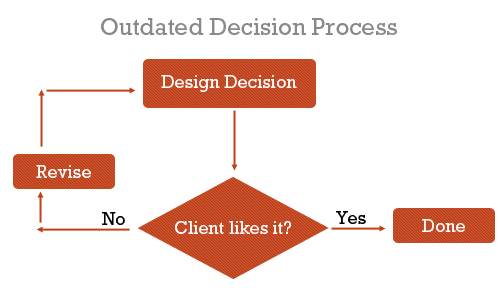
\includegraphics[scale=0.5]{OutDatedDecisionProcess.jpg}
\caption{old decision process, Jacob Gube 2010}
\end{figure}
nowhere in the design process is the users a factor, the design was simply made according to how the designers as well as the client felt it should be. making the same kind of chart for a user-centered approach could look like:\\
\begin{figure}[H]
\centering
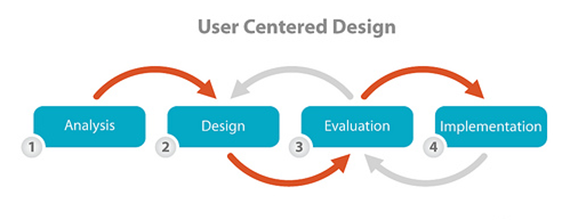
\includegraphics[scale=0.5]{UserCenteredDesign.png}
\caption{a chart of how user-centered design could function, Usabilla 2014}
\end{figure}
as this chart shows user-centered design can be an iterative process. the grey arrow represents the user feedback, which shows that the users should be involved in the evaluation of a design. This method can be overwhelming if the evaluation is only being done on implemented prototypes.

User Experience and usability is often confused since a large portion of the guidelines for proper usability also applies to giving a good user experience. What sets the user experience apart from usability is the feelings that the user is subjected to while using the site/app/programme.
An example of which could be the iBooks app for iPad, which is basically an application for reading and browsing E-books. The layout is simple,  it provides an overview of the owned books with a visual representation of the covers which is common for such apps and as such do not set itself apart from the state of the art when it comes to usability, however the user experience is greatly improved simply by changing the background to resemble a bookshelf, it gives a “cozy” feel to the app, you can almost imagine yourself sitting in front of the fireplace sitting with a good book.

\begin{figure}[h!]
\centering
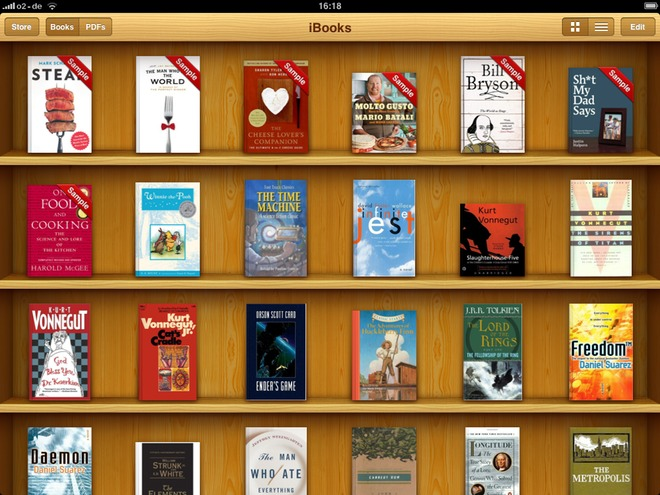
\includegraphics[scale=0.5]{iBooks.png}
\caption{Apple iBooks}
\end{figure}\todo{this needs a caption}

\begin{figure}[h!]
\centering
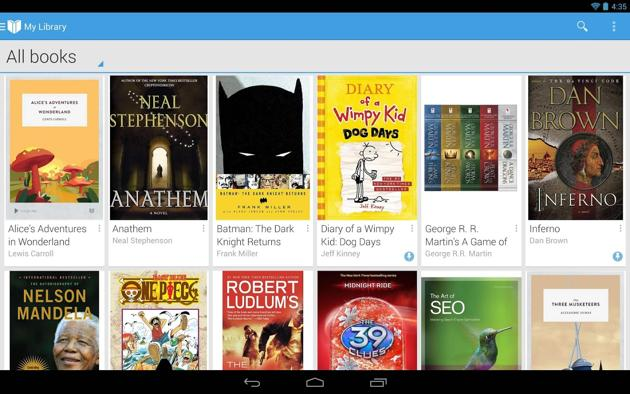
\includegraphics[scale=0.5]{GooglePlayBooks.png}
\caption{Google Play Books}
\end{figure}
\subsection{User experience for mobiles}
when designing a mobile app with UX focus, the unique challenges of the mobile platform has to be considered. A brief look at two of the most outstanding difficulties:
\begin{itemize}
\item Screen size\\
as opposed to a traditional computer screen the general mobile platform has a much more limited amount of screen space. This restriction will force the designers to eliminate as many redundancies as possible so as to not clutter the screen with unnecessary information. \cite{Sardo}
\item User input\\
user input is according to Giorgio Sardo one of  the smartphones weakness. it is mentioned that “Entering text on a mobile phone is hard, and people tend to avoid it if they can”\cite{Sardo}
\item Loading times\\
Mobile devices are generally slower than a PC or Mac, both when it comes to processing power and internet speed, assuming they’re using a mobile network [ref. mobile usability jakob nielsen/raluca budui 2013]. 
\end{itemize}
When attempting to improve usability and user experience, for people using a site or a programme on a phone, the optimal way to do so is to make an actual app where you either port the mobile site or the web application so that it can be downloaded and accessed directly from your phone or tablet instead of via the internet browser. 
Some of the guidelines for optimizing for mobile devices are cutting features, reduce word count and enlarge interface elements to accommodate the “fat finger problem”.[ref. mobile usability jakob nielsen/raluca budui 2013] an example of poor simplification used in the book is IKEA [ikea screenshot from the book] where they simplify the mobile site by only showing a single item when browsing for bedframes.
\subsection{Understanding our Users}
Even though have previously analysed out target group, when we want to focus on the user experience, further target group considerations has to be made, that is why this paper will next talk about the concept of understanding the users. Georgi Sardo provides three points that will help with the design process of the app:
\begin{itemize}
\item What are your users’ digital device skills? Are they used to working with digital devices and software applications?\cite{Sardo}
\item What are your users’ skills in using your application? Does the application revolve around their professional area?\cite{Sardo}
\item Is the application the focal point for your users? Or is their attention limited?\cite{Sardo}
\end{itemize}
these three points can help develop an app that will be focused on the users needs, which is at its core what UX is all about.